Plot these data and find the equation of the least squares line, $y=a+bx$. Suppose a cricket of this
species is observed to chirp eighteen times per second. What would be the estimated temperature?\\\\

\begin{solution}\renewcommand{\qedsymbol}{}\ \\
    Well, given the sums, we have that $\beta_0=25.2323$ and $\beta_1=3.2911$ by Cramer's Rule. So, we
    have the least squares line $y=25.2323+3.2911x$. So, at $18$ chirps per second, we would expect the
    tempurature to be $84.47$ degrees fahrenheit.\\

    \begin{center}
        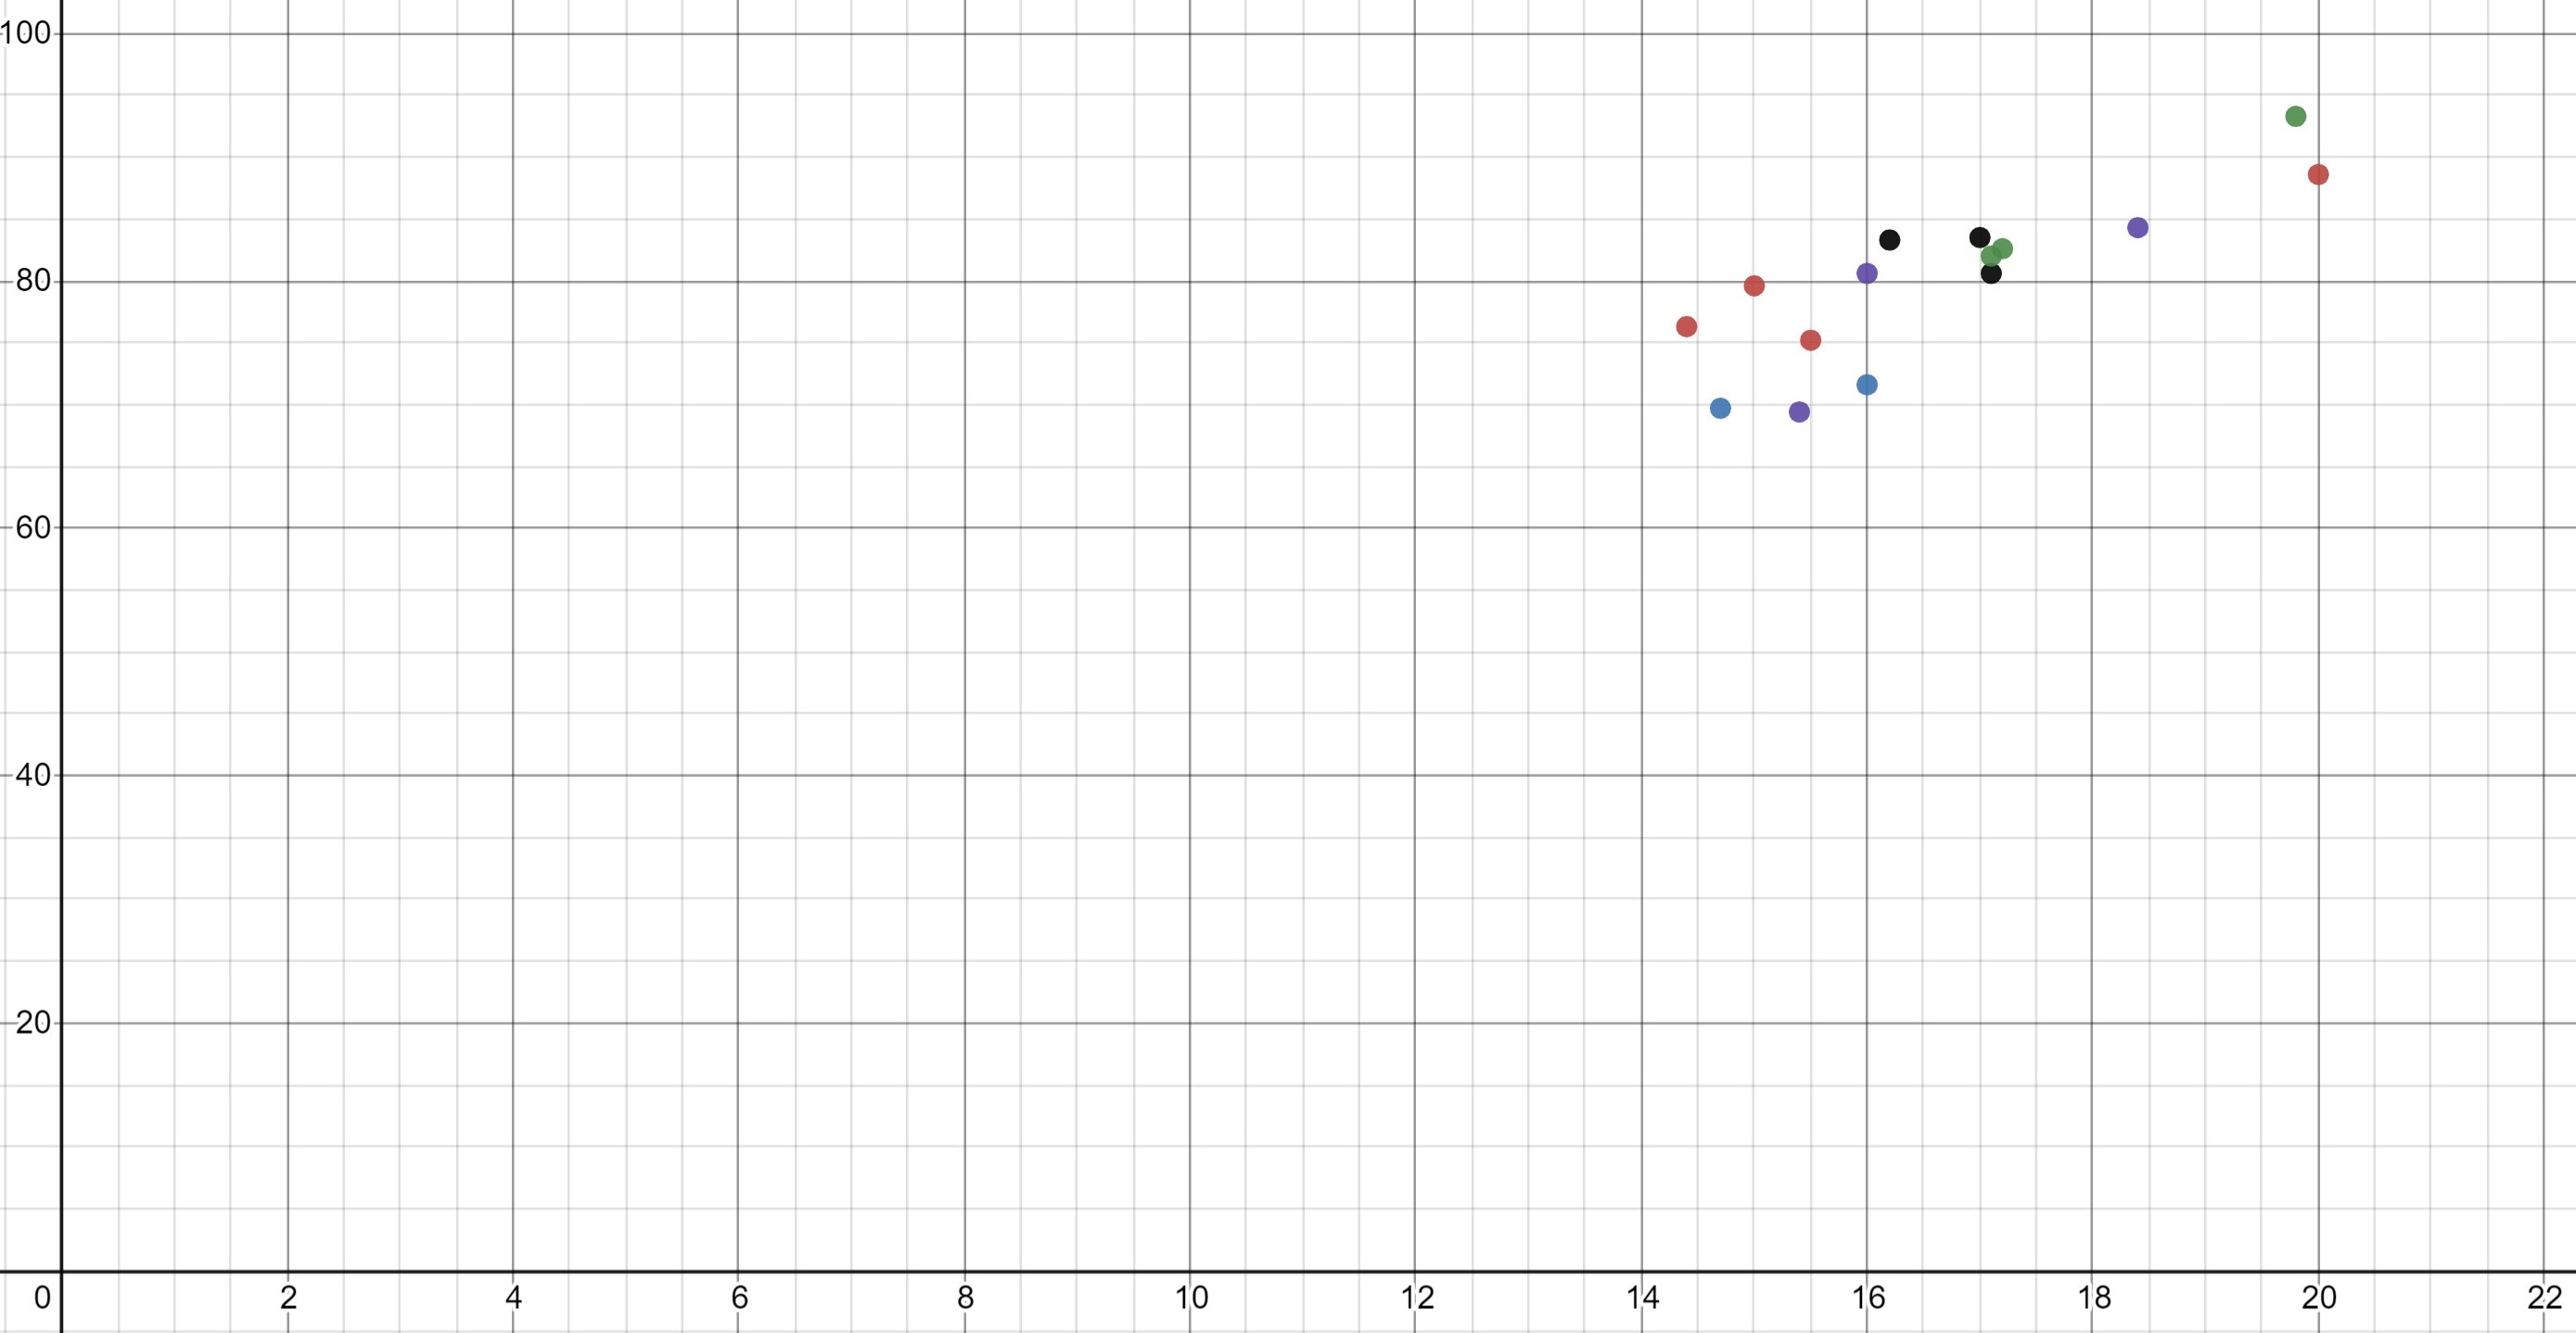
\includegraphics[scale=0.5]{11-2-1.JPG}
    \end{center}

\end{solution}